%----------------------------------------------------------------------------------------------------------------------

\begin{frame}{Part I}
\centering \textbf{\Large Sheet Metal Solid to Midsurface Transformation}
\end{frame}

\begin{frame}{Cellular Decomposition}
\begin{itemize}[noitemsep,label=\textbullet,topsep=2pt,parsep=2pt,partopsep=2pt]
\item Given a Sheet Metal solid, 
\item Come up with the dimension-reduction-transformation equations 
\item for predicting topological entities of its corresponding Midsurface. 
\item The given solid model is first decomposed into volumes
\item Then the dimension-reduction-transformation is derived. 
\item Topology by the decomposition is called {\em Cellular Topology}.  
\item Many commercial \& academic methods are available% \cite{BidarraKrakerBronsvoort1998, Woo2003, Chong2004, Cao2011, Boussuge2013}. 
\end{itemize}

\vspace{-5mm}

\begin{center}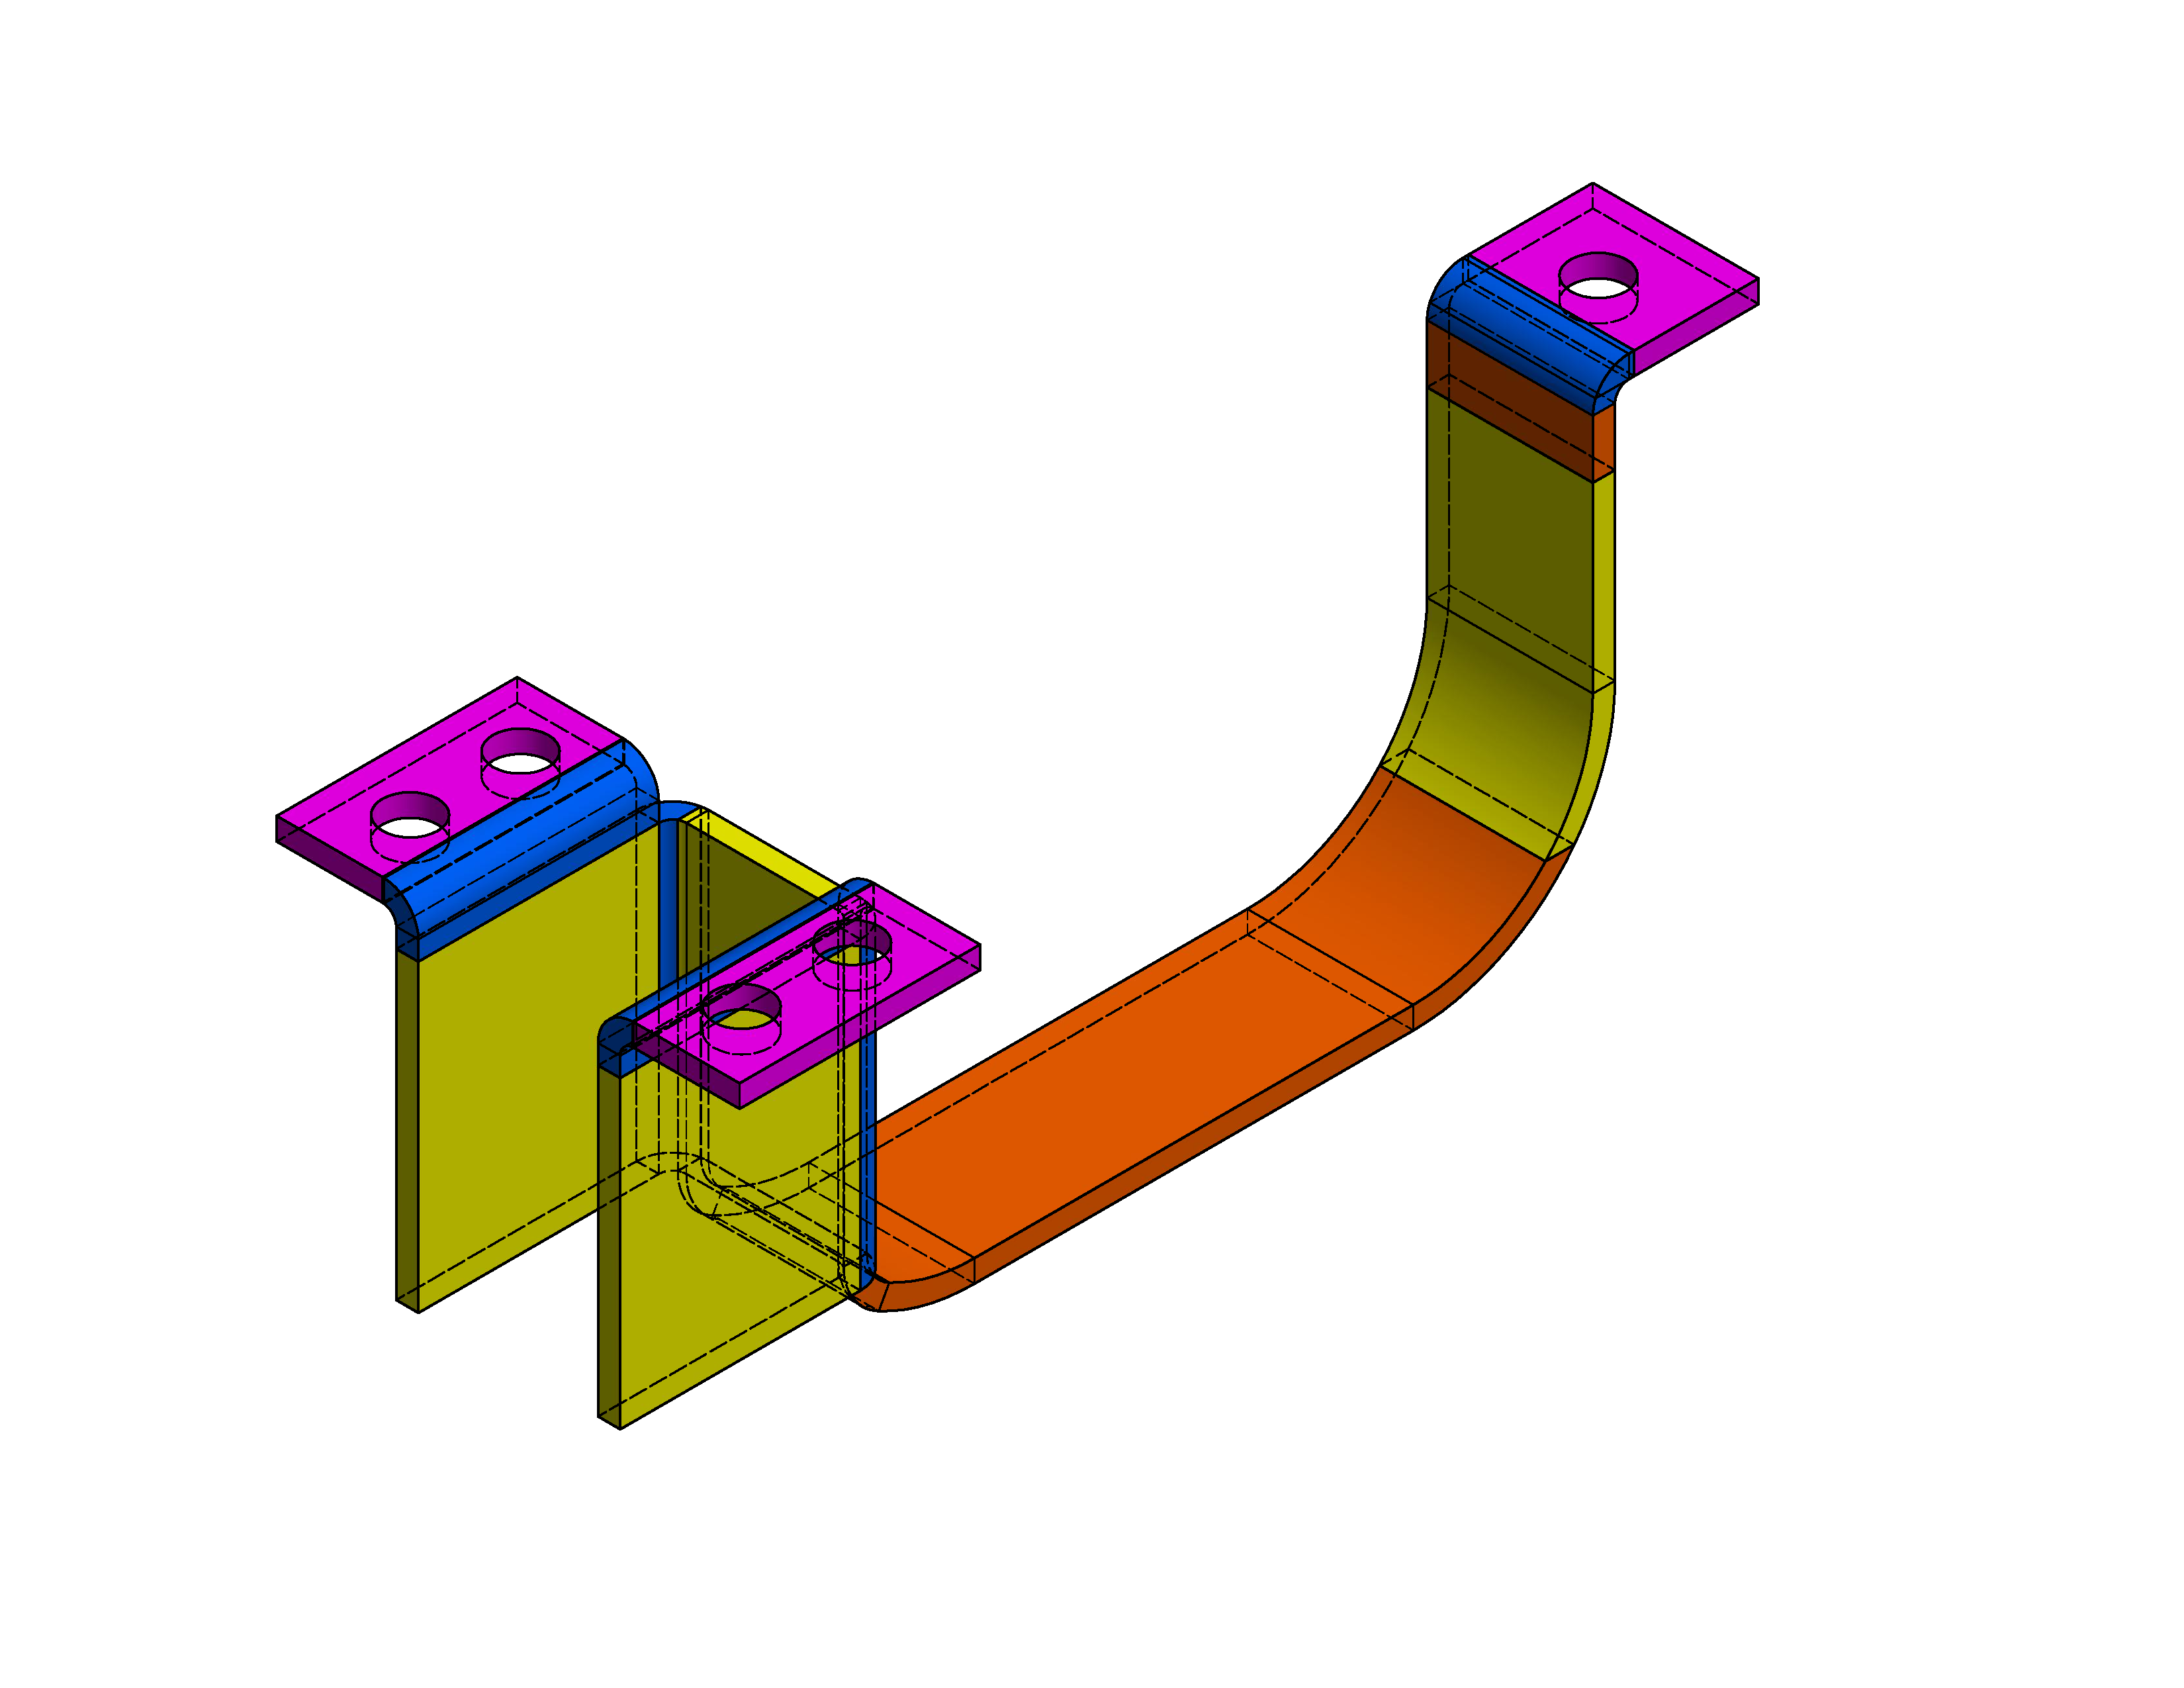
\includegraphics[width=0.4\linewidth]{../Common/images/VolDecomp1.pdf}\end{center}

\vspace{-3mm}

\end{frame}


\begin{frame}{What is a Cell?}

%\resizebox{0.9\linewidth}{!}{
%\begin{tabular}[h]{@{} p{0.35\linewidth}  p{0.6\linewidth}@{}}

\begin{itemize}[noitemsep,label=\textbullet,topsep=2pt,parsep=2pt,partopsep=2pt]
\item The  fundamental unit is called $Cell$,
\item Has dimensionality $0,1,2,3$ 
\item Adjacency to its neighbors is $Cell_{dimension,adjacency}$ 
\item Actual size and shape depends on underlying geometry. 
\end{itemize}
%\begin{center}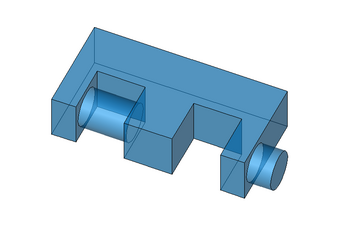
\includegraphics[width=0.8\linewidth]{../Common/images/CellsACIS}\end{center}
%&

%\raisebox{-0.9\height}{
\resizebox{\linewidth}{!}{
\begin{tabular}[h]{@{}p{0.1\linewidth} p{0.1\linewidth} p{0.4\linewidth} p{0.4\linewidth}@{}} 

$Cell_{3,*}$  & 
\adjustbox{valign=t}{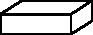
\includegraphics[width=\linewidth]{../Common/images/SimplePlate1.pdf}} &
3D cells, solids, topologically similar to a simple plate &
 $faces=6 \newline edges=12 \newline vertices =8$ \\
 
 $Cell_{2,*}$ &
 \adjustbox{valign=t}{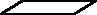
\includegraphics[width=\linewidth]{../Common/images/SimplePlane1.pdf}} &
  2D cells, topologically similar to a planar surface  &
   $faces=1 \newline edges=4 \newline vertices =4$ \\
   
$Cell_{1,*}$ &
 \adjustbox{valign=t}{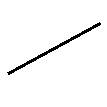
\includegraphics[width=\linewidth]{../Common/images/SimpleLine1.pdf}} &
1D cells, topologically equivalent to a line &
 $edges=1  \newline vertices =2$ \\
 
 $Cell_{3,h}$ &
  \adjustbox{valign=t}{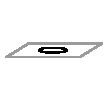
\includegraphics[width=\linewidth]{../Common/images/SimpleHole1.pdf}} &
  Hole is assumed to be cylindrical through-all (true for Sheet Metal parts) &
   $edges=1  \newline vertices =1$ \\

 \end{tabular}

}\\

%\end{tabular}
%}
\end{frame}



\begin{frame}{Cellular Topology}
\begin{tabular}{@{}p{0.6\linewidth}p{0.35\linewidth}@{}}

\begin{itemize}[noitemsep,label=\textbullet,topsep=2pt,parsep=2pt,partopsep=2pt]
\item Decomposition introduces new interface boundaries
\item intersection-volumes or touching boundaries are called interface-Cells, which can be 3D (solids) or 2D (faces) , respectively. 
\item Prefix $s$ is applied in case the $Cell$ is from {\em original solid}, $i$ in case it is of newly introduced  {\em interface} type, and $m$ for {\em Midsurface} cells.

\end{itemize}

\begin{tabular}[htp]{@{}p{0.48\linewidth} p{0.48\linewidth}@{}} 
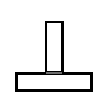
\includegraphics[width=0.6\linewidth]{../Common/images/Interface2d.pdf} 
\label{fig_interfaces} &
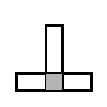
\includegraphics[width=0.6\linewidth]{../Common/images/Interface3d.pdf} \\
2D Interface & 3D Interface\\
\end{tabular}

&

\raisebox{-0.9\height}{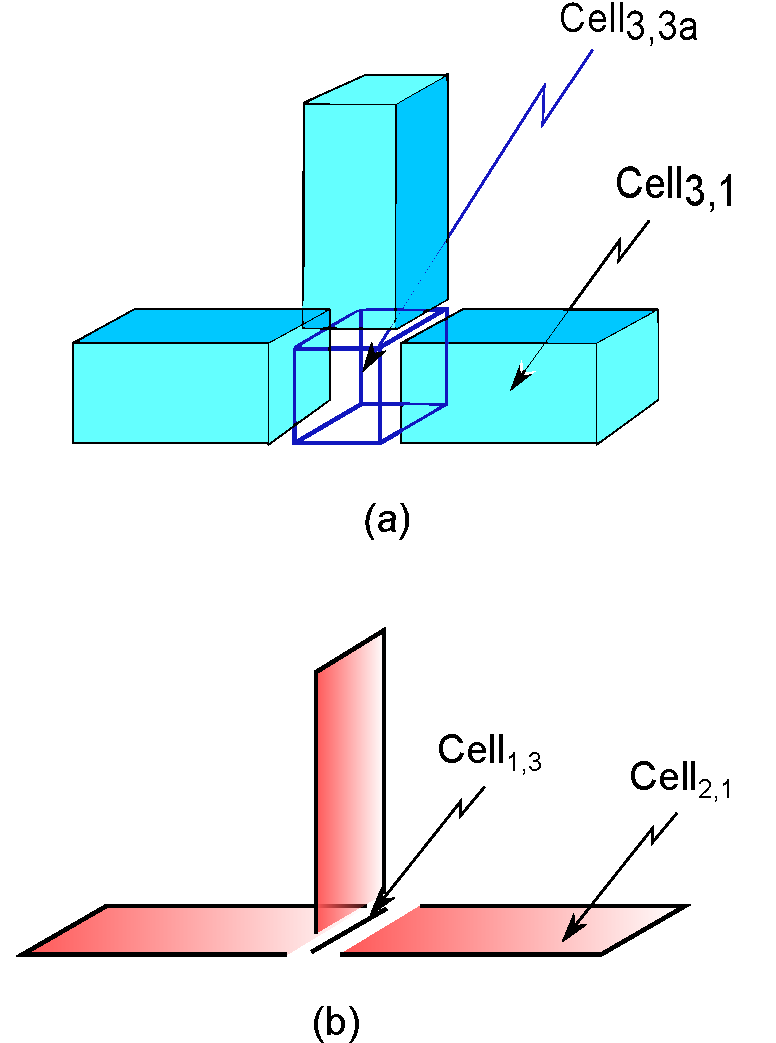
\includegraphics[width=\linewidth]{../Common/images/Cellular_Topology.pdf}}\\
\end{tabular}
\end{frame}

\begin{frame}{Steps:Topological dimension reduction}
From Solid-3D-Cells to Midsurface-2D-Cells:

\begin{itemize}[noitemsep,label=\textbullet,topsep=2pt,parsep=2pt,partopsep=2pt]
%[noitemsep,topsep=2pt,parsep=2pt,partopsep=2pt]

	\item  $sCell_{3,n}$:	Solid Cell with $n$ touching sides transforms into Midsurface Cell   $mCell_{2,n}$, a surface having $n$ empty edges. 
\begin{equation}
f=1,
e=4-n,
v=4-2n
\label{eqn_cellularna}
\end{equation} 

	\item   $sCell_{3,h}$ : Negative solid  Cell representing a through hole transforms into Midsurface Cell  $mCell_{2,h}$, a hole in the surface.
\begin{equation}
e=1, v=1
\label{eqn_cellularah}
\end{equation} 

	\item $iCell_{3,n}$ :	Interface Solid Cell with $n$ adjacent touching sides transforms into Midsurface Cell  $mCell_{1,n}$, a radial edge with $n$ leaves. 
\begin{equation}
e=1,
v=2
\label{eqn_cellulara}
\end{equation}

	\item  $iCell_{2,2}$ :	Interface Face Cell being touched from both sides  transforms into Midsurface Cell  $mCell_{1,2}$, a radial edge with 2 leaves. 
\begin{equation}
e=1,
v=2
\label{eqn_cellularaf}
\end{equation}
\end{itemize}
\end{frame}

\begin{frame}{Examples}
\resizebox{0.7\linewidth}{!}{
\begin{tabular}[h]{@{}p{0.1\linewidth} p{0.1\linewidth}  p{0.15\linewidth}  p{0.15\linewidth}  p{0.35\linewidth}@{}} \toprule
{\bf Solid} & {\bf mSurf}  & {\bf sCells} & {\bf mCells}  & {\bf Predicted Entities} \\ \midrule  

\adjustbox{valign=c}{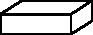
\includegraphics[width=\linewidth]{../Common/images/SimplePlate1.pdf}}  &  
\adjustbox{valign=c}{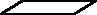
\includegraphics[width=\linewidth]{../Common/images/SimplePlane1.pdf}} &  
$sCell_{3,0}$ & $ mCell_{2,0}$ & 
$ 1f+(4-0)e+(4- 2\times 0)v \newline = 1f+4e+4v$
\\ %\midrule

\adjustbox{valign=c}{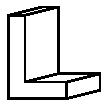
\includegraphics[width=\linewidth]{../Common/images/LPlate1.pdf}}  &  
\adjustbox{valign=c}{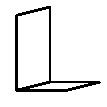
\includegraphics[width=\linewidth]{../Common/images/LPlane1.pdf}} &  

$2 \times sCell_{3,1} \newline + iCell_{3,2}$ & $2 \times mCell_{2,1} \newline + mCell_{1,2}$  & 
$ 2 \times (1f + (4-1)e+(4-2\times 1)v ) \newline + (1e + 2v) \newline = 2f+7e+6v$ 
\\ %\midrule


\adjustbox{valign=c}{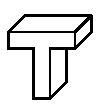
\includegraphics[width=\linewidth]{../Common/images/TPlate1.pdf}}  &  
\adjustbox{valign=c}{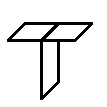
\includegraphics[width=\linewidth]{../Common/images/TPlane1.pdf}} &  

$3 \times sCell_{3,1} + iCell_{3,3}$   &  $3 0.8\times mCell_{2,1}  + mCell_{1,3}$  & 
$3 \times (1f+(4-1)e+ (4-2\times 1)v)  + (1e+2v)  = 3f+10e+8v$ 
\\ %\midrule

\adjustbox{valign=c}{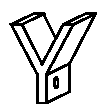
\includegraphics[width=\linewidth]{../Common/images/YwithHole1.pdf}}  &  
\adjustbox{valign=c}{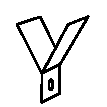
\includegraphics[width=\linewidth]{../Common/images/YwithHolem1.pdf}} &  

$3 \times sCell_{3,1}  + iCell_{3,3}  + sCell_{3,h}$   &  
$3 \times mCell_{2,1}  + mCell_{1,3}  + mCell_{2,h}$  & 
$3 \times (1f+(4-1)e+ (4-2\times 1)v)  + (1e+2v)  + (1e+1v)  = 3f+11e+9v$
\\ %\midrule

\adjustbox{valign=c}{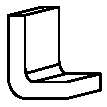
\includegraphics[width=\linewidth]{../Common/images/LwithRound1.pdf}}  &  
\adjustbox{valign=c}{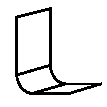
\includegraphics[width=\linewidth]{../Common/images/LwithRoundm1.pdf}} &  

$2 \times sCell_{3,1}  + 2 \times  iCell_{2,2}  + sCell_{3,2}$   &  
$2 \times mCell_{2,1}  + 2 \times mCell_{1,2}  + mCell_{2,2}$  & 
$2 \times (1f+(4-1)e+ (4-2\times 1)v)  + 2 \times (1e+2v)  + (1f+(4-2)e+ (4-2\times 2)v)  = 3f+10e+8v$
\\ 

\bottomrule
\end{tabular}
}

\vspace{2mm}
Predicted Midsurface entities match with the actual ones!!!
\end{frame}

\begin{frame}{Practical Example}
\begin{center}
\resizebox{0.5\linewidth}{!}{

\begin{tabular}[htp]{@{}p{0.48\linewidth} p{0.48\linewidth}@{}} 
{\bf Solid} & {\bf Cellular Classification} \\
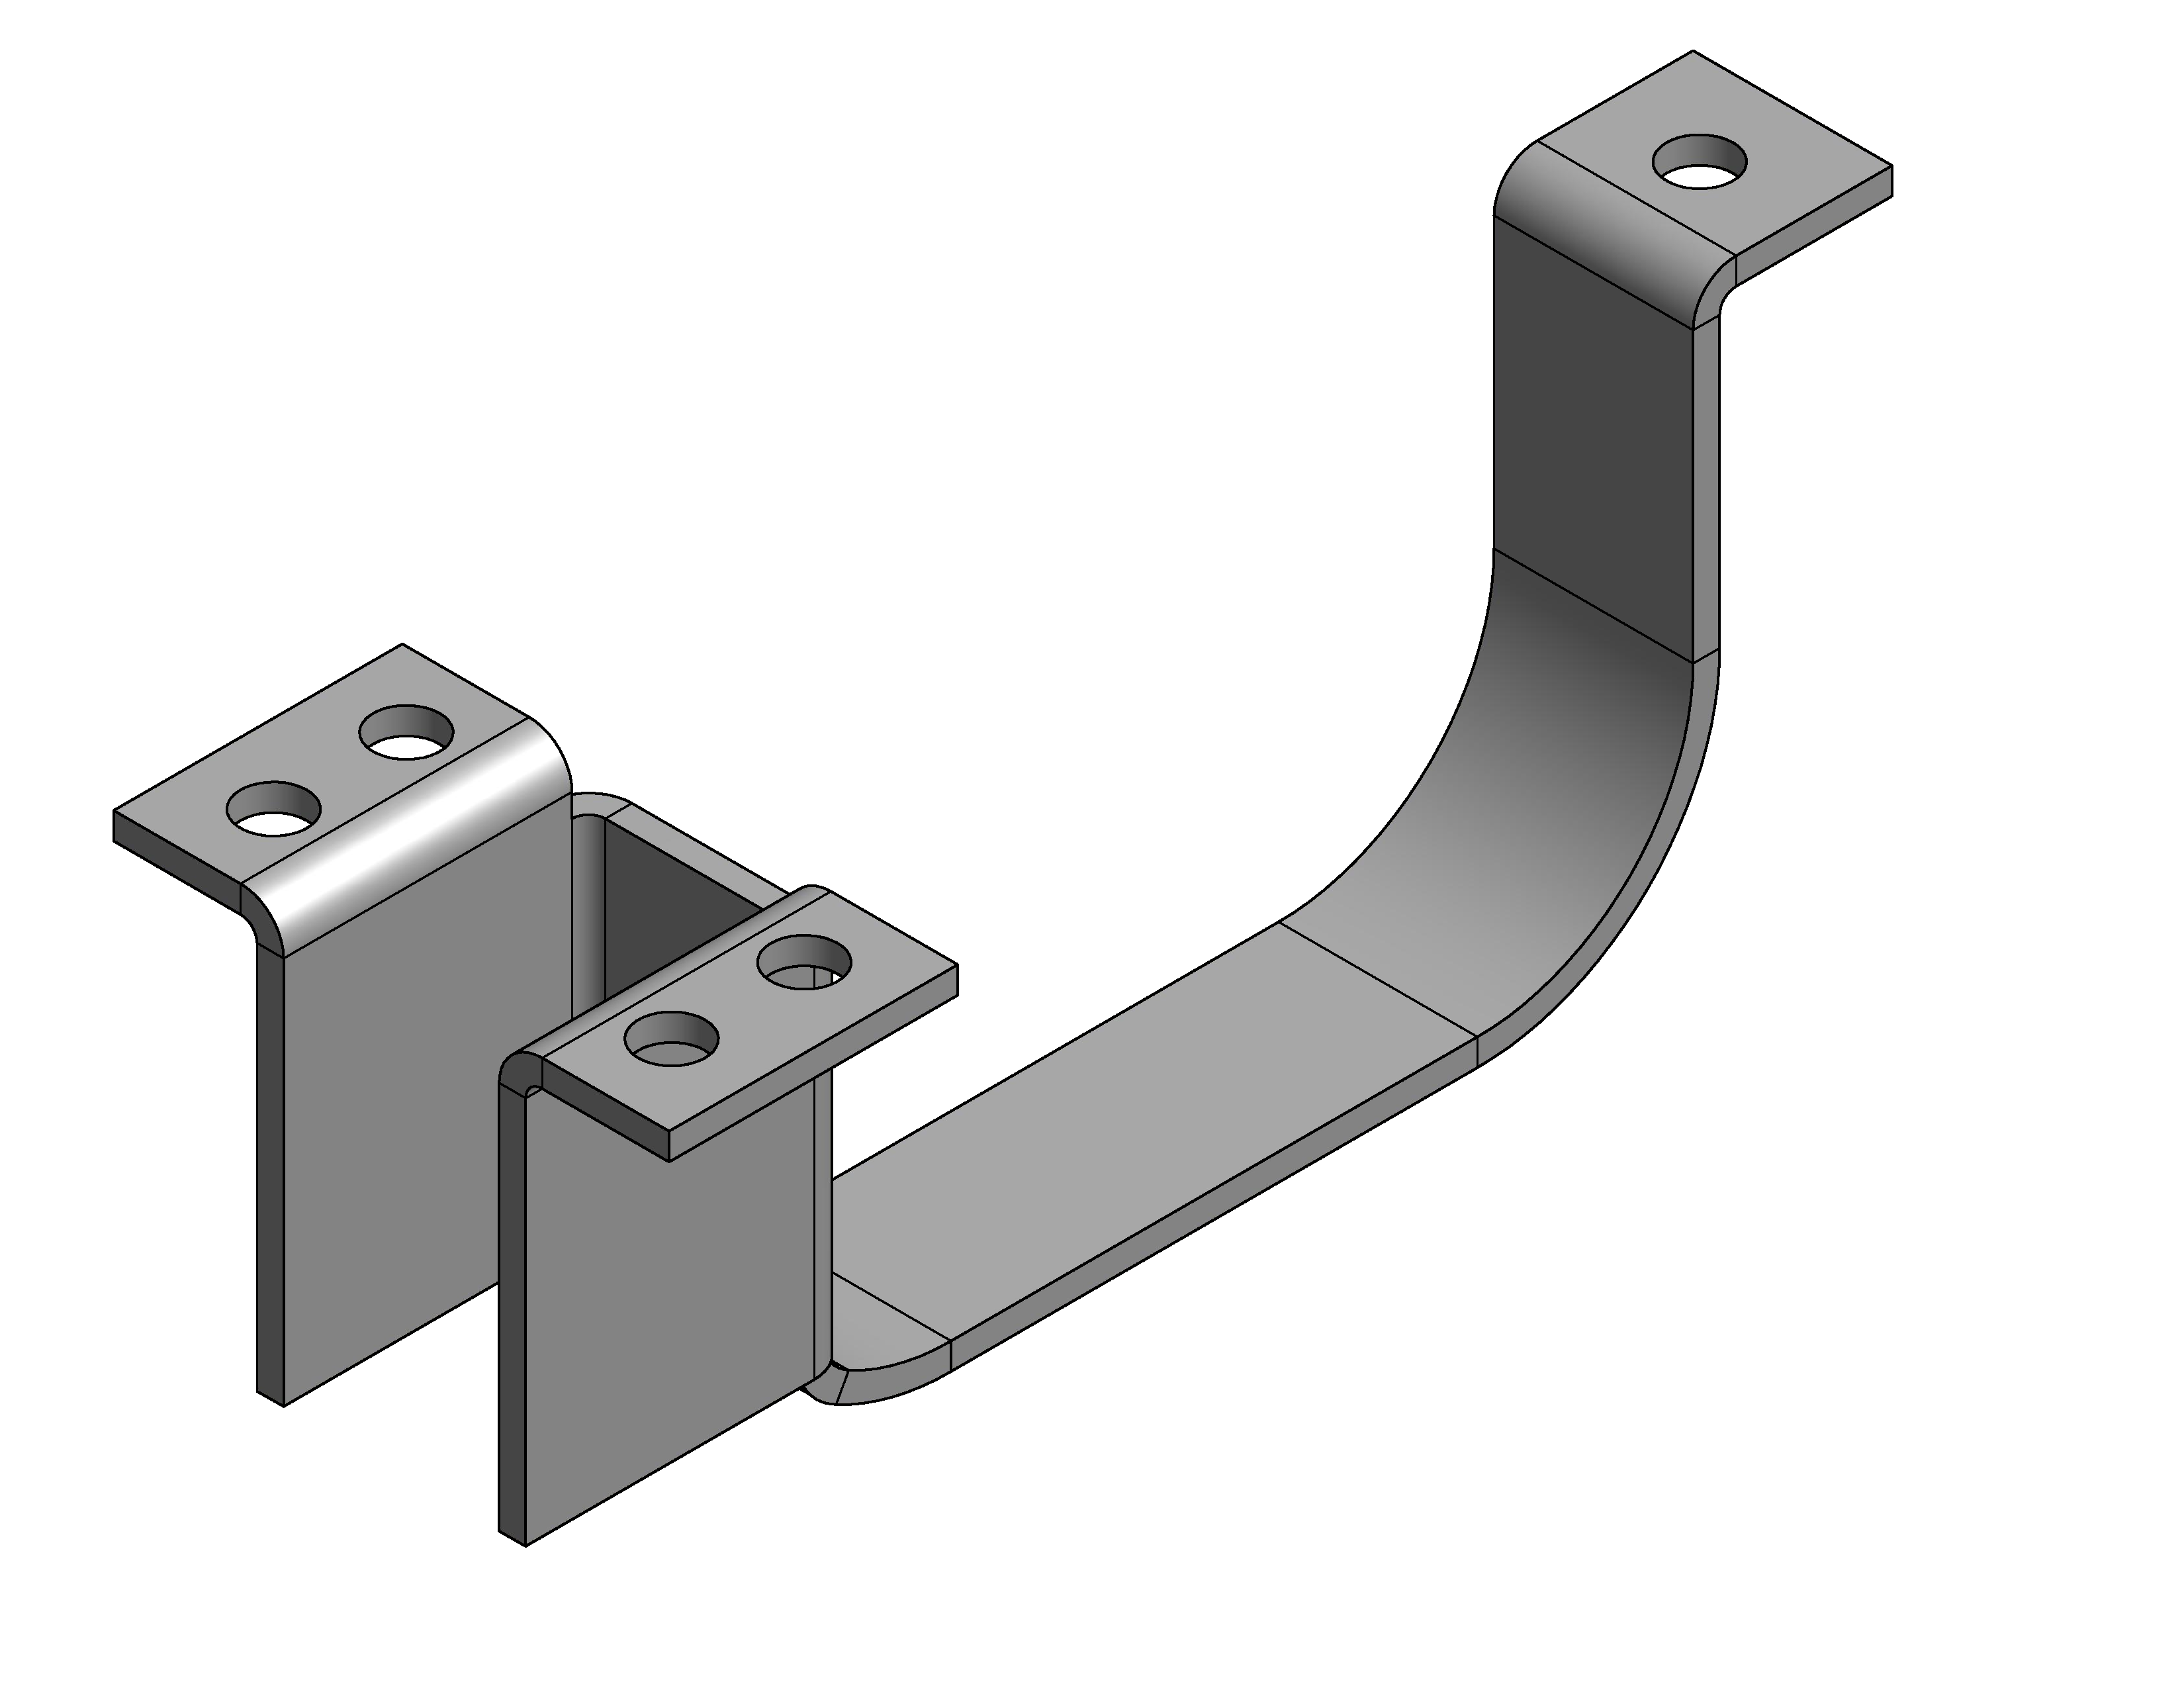
\includegraphics[width=\linewidth]{../Common/images/SimpleBracketshaded.pdf} &
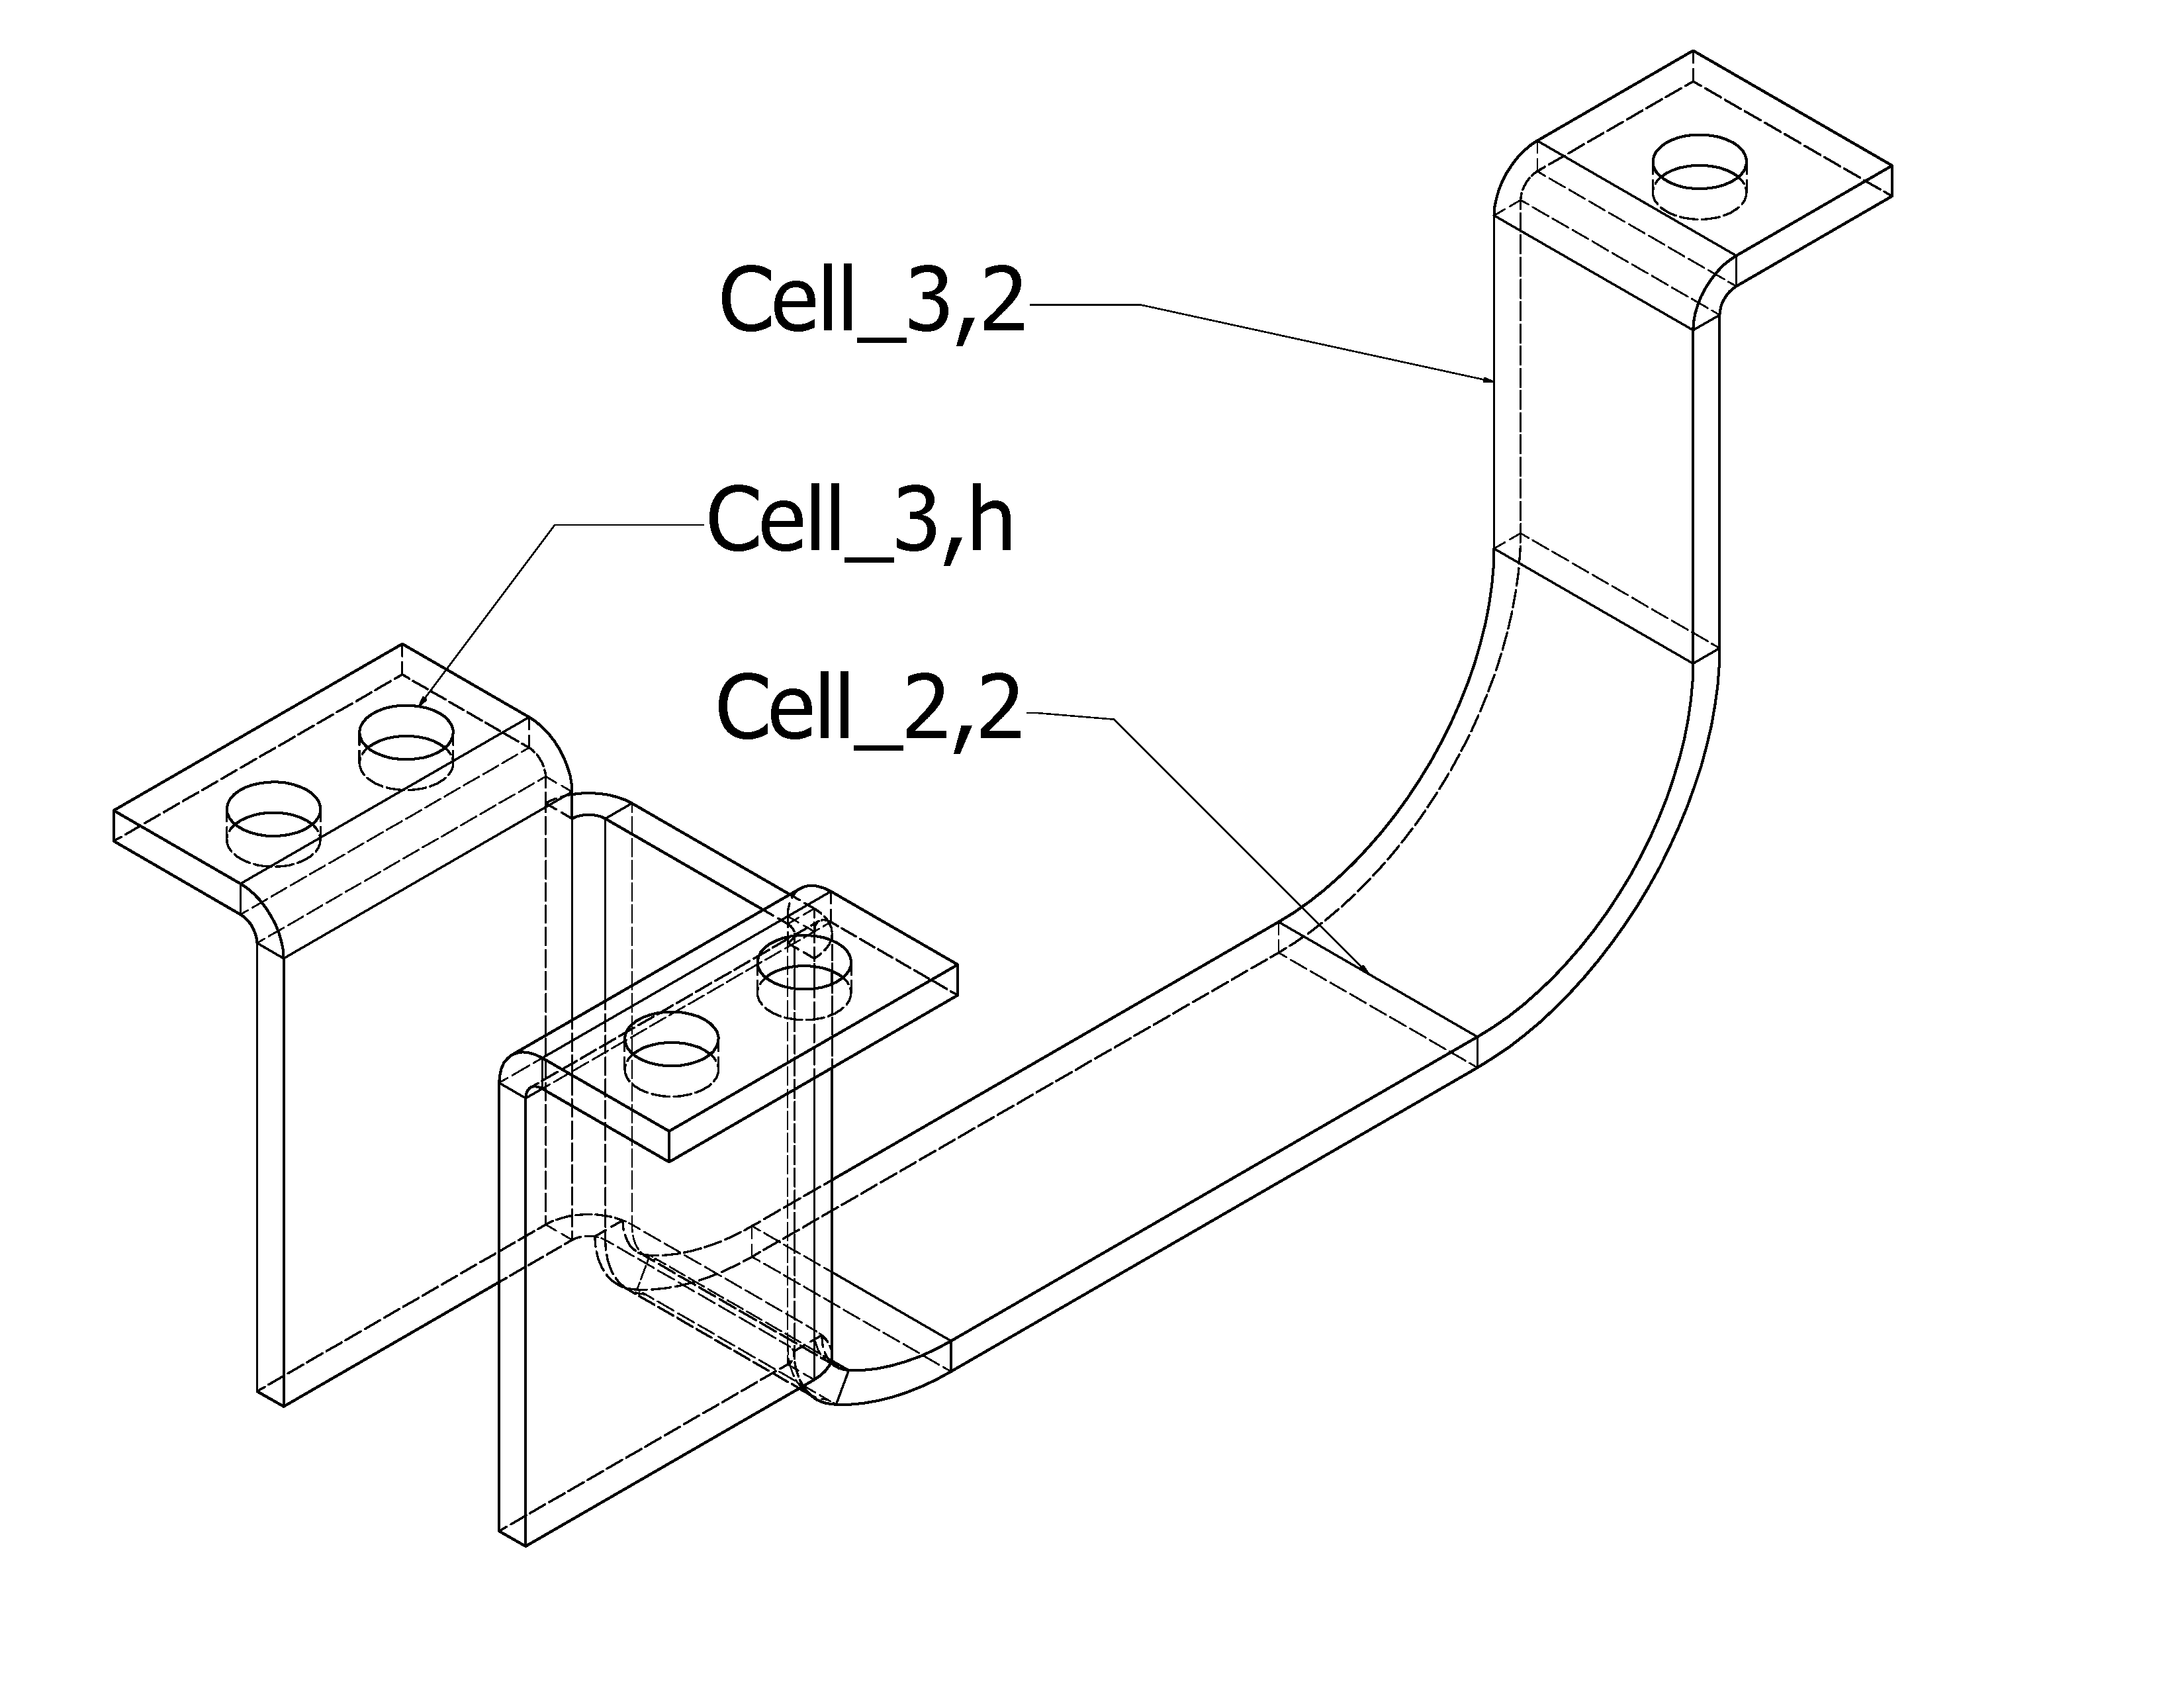
\includegraphics[width=\linewidth]{../Common/images/SimpleBracket.pdf}\\
\end{tabular}

}
\end{center}
\begin{itemize}[noitemsep,label=\textbullet,topsep=2pt,parsep=2pt,partopsep=2pt]
%[noitemsep,topsep=2pt,parsep=2pt,partopsep=2pt,leftmargin=*]
	\item \textbf {Solid Cells}: \newline  $5 \times sCell_{3,h} + 3 \times sCell_{3,1} + 13 \times sCell_{3,2} + 14 \times iCell_{2,2} $
	\item \textbf {Transformed Midsurface Cells}: \newline $5 \times mCell_{2,h} + 3 \times mCell_{2,1} + 13 \times mCell_{2,2} + 14 \times mCell_{1,2}$
	\item \textbf {Predicated Midsurface entities are}:  \newline $5(1e+1v) + 3 (1f+3e+2v) + 13 (1f+2e+0v) + 14(1e+2v) = 
16f + 54e + 39v$
\end{itemize}
The Proposed derivation (Eqn   \ref{eqn_cellulara}, \ref{eqn_cellularaf}, \ref{eqn_cellularna}, \ref{eqn_cellularah} ) predicts Midsurface topological entities, validates the non-manifold equation (Eqn \ref{eqn_nonmanifold}) with $s=1, r=5, h=5$. Both sides: $ 39 - 54 + (16 -5) = 1 (1-5)$

\end{frame}

\begin{frame}{Part II}
\centering \textbf{\Large Midsurface to Sheet Metal Solid Transformation}
\end{frame}

\begin{frame}{Midsurface to Sheet Metal Solid Transformation}
\begin{itemize}[noitemsep,label=\textbullet,topsep=2pt,parsep=2pt,partopsep=2pt]
\item Given a Midsurface of a Sheet Metal Solid
\item Topological entities  of its corresponding Sheet Metal solid are predicted
\item They are verified with Manifold equation (Eqn \ref{eqn_manifold}).
\item Topology Midsurface contains far richer (classifiable) information 
\item For example, Midsurface of 'T' shaped solid, which can be represented as Figure \ref{fig_nonmanifold}
\end{itemize}

\begin{figure}[htbp]
\begin{center}
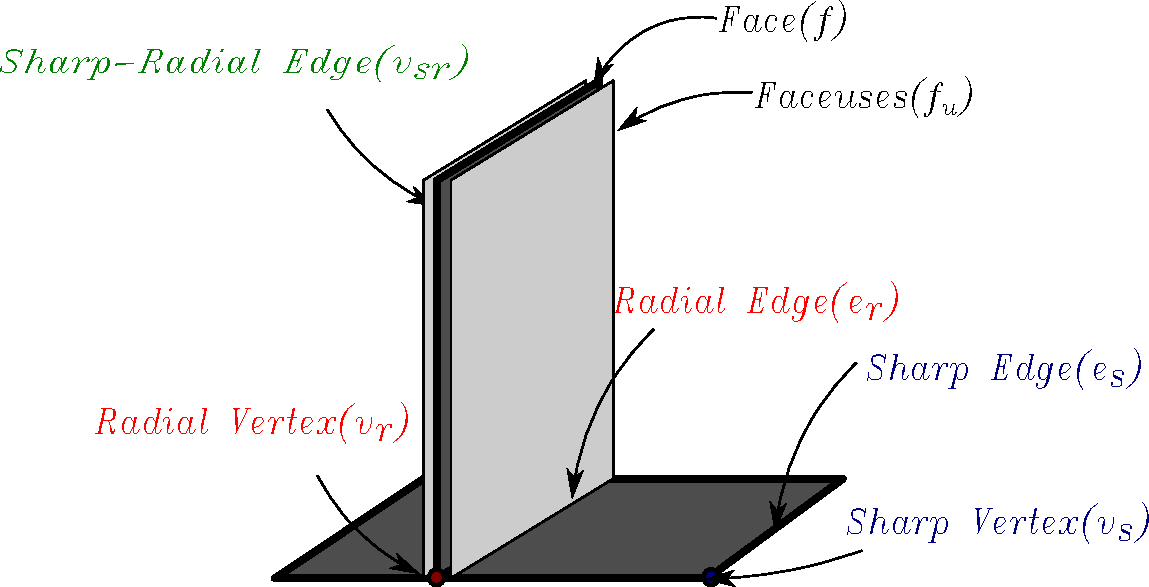
\includegraphics[width=0.4\linewidth]{../Common/images/NonManifoldT1.pdf} 
\end{center}
\caption{Classification of topological entities of the Midsurface}
\label{fig_nonmanifold}
\end{figure}
\end{frame}

\begin{frame}{Classification of topological entities of the Midsurface}
	\begin{itemize}[noitemsep,label=\textbullet,topsep=2pt,parsep=2pt,partopsep=2pt] 
%	[noitemsep,topsep=2pt,parsep=2pt,partopsep=2pt,label={}]\label{list_topos}
	\item Faces ($f$): Bound by two face-uses $f_u$.
	
	\item Sharp Vertex ($v_s$): Connected to two edges of the same face
	\item Sharp Edge ($e_s$): Connected to two sharp vertices

	\item Radial Vertex ($v_{r}$): Connected edges of different faces
	\item Degree ($n_{r}$) at the radial edge is the number of faces attached to it 
	\item Cross Radial Edge ($e_{r}$): Connected between two radial vertices, connects two different faces
	\item Side-Radial  Edge ($e_{rr}$): Connected between two radial vertices, is of same face
	\item Sharp-Radial Edge ($e_{sr}$): Between sharp and radial vertex
	\item Internal Edge ($e_i$): Part of the inner loop
	\item Internal Vertex ($v_i$):Connected to internal edge
	\item Internal Loop ($r_i$) : Internal edges and vertices
	\end{itemize}
\end{frame}


\begin{frame}{Steps: Topological dimension addition}
Sheet Metal part can be imagined to be thickened Midsurface \cite{SHLee2001}.
\begin{tabular}[htp]{@{}p{0.75\linewidth} p{0.2\linewidth}@{}} 

	\begin{itemize}[noitemsep,label=\textbullet,topsep=2pt,parsep=2pt,partopsep=2pt]
%	[noitemsep,topsep=2pt,parsep=2pt,partopsep=2pt,leftmargin=*]
	\item Face-uses become Principal Faces. 
 
\item Sharp vertices create capping edges

%\item Face-uses around a radial edge remain as connected in the solid as well. 
%Face-uses of same face will get connected via thickness faces
\item A new loop is proposed for side-capping faces. 
\item Loop between two Sharp Vertices ($v_s$) via more than one Sharp  ($e_{sr}$) or Side Radial ($e_{rr}$) edges but not via the Cross Radial edge ($e_r$). 
\item Such independent paths creating side faces: $l_p$.

	\item Loop between two $v_s$, gives a capping face  (a)
	\item Loop between three $v_s$, branched gives a combined capping face (b)
	\item Loop between two $v_s$ with multiple $e_{sr}$ in between. gives a combined capping face (c)
	\end{itemize}
	&
\adjustbox{valign=t}{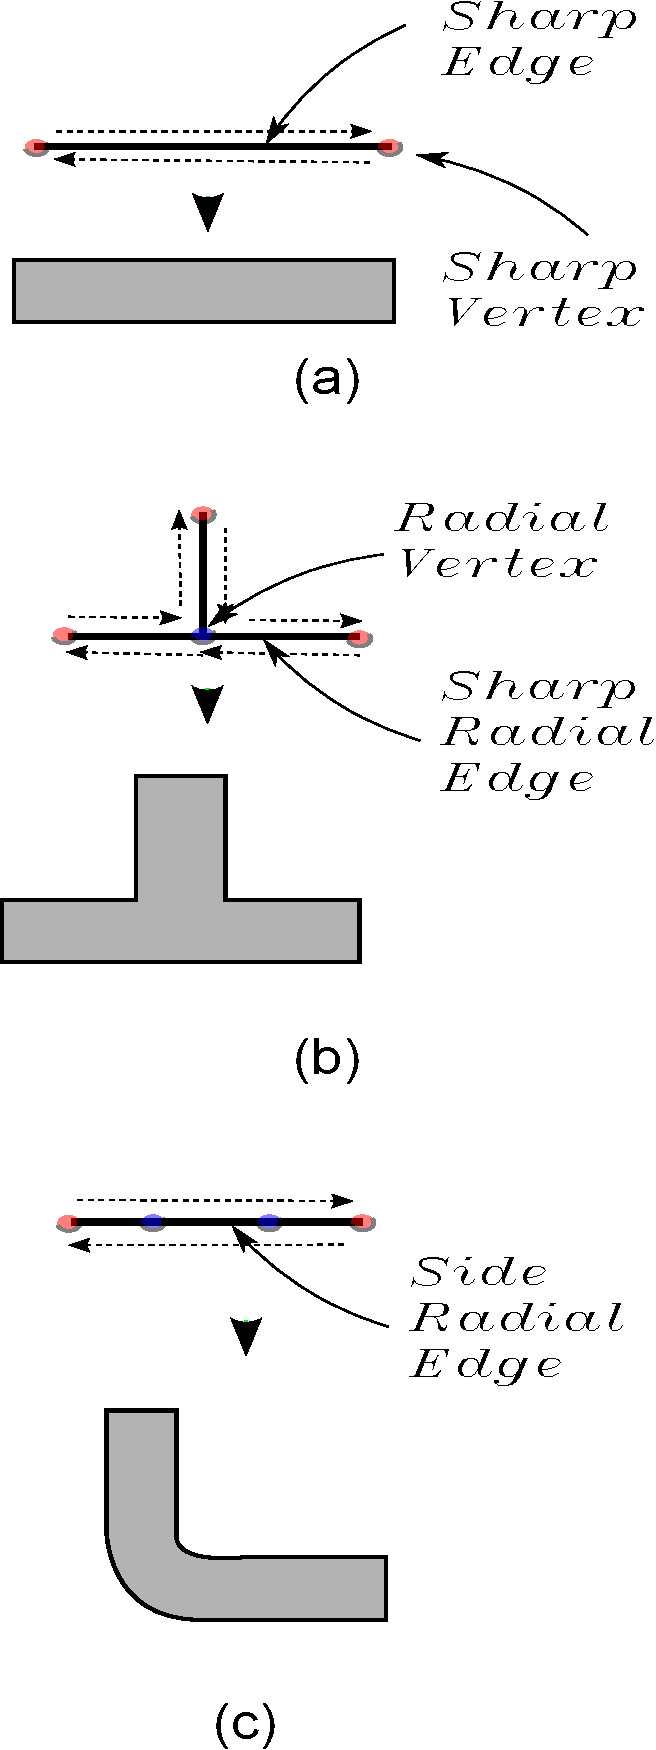
\includegraphics[width=\linewidth]{../Common/images/NonManifoldLoopsToFaces1.pdf}} \\
\end{tabular}



	

%\item Radial vertices or edges won't create any new topological entity
%\end{itemize}

\end{frame}

\begin{frame}{Prediction of Topological entities in the thickened solid}


\begin{itemize}[noitemsep,label=\textbullet,topsep=2pt,parsep=2pt,partopsep=2pt]
%[noitemsep,topsep=2pt,parsep=2pt,partopsep=2pt,label=\textbullet]
\item Manifold-Vertices  ($v_m$) 
%= Double the sharp and internal vertices (one up, one below) + vertices for junctions (summation of  number radial vertices times their  degrees)
\begin{equation}
v_m = 2 (v_s + v_i) + \sum n_{r} v_{r} \label{eqn_vm}
\end{equation}
\item Manifold-Edges ($e_m$)
%= 2 times sharp, sharp-radial and internal edges (offset up and down) + degree times radial edges for offsets at junctions + sharp vertices for vertical capping edges + internal vertices for vertical seam edges
\begin{equation}
e_m = 2 (e_s + e_{sr} + + e_{rr} + e_i) + \sum n_r e_r  + v_s + v_i\label{eqn_em}
\end{equation}
\item Manifold-Faces ($f_m$) 
%= Double the faces (offset up and down) + sharp edges for capping faces + paths to have one combined face + internal edges for capping internal faces
\begin{equation}
f_m = 2f + e_s + l_p + e_i \label{eqn_fm}
\end{equation}
\item Manifold-Shells ($s_m$) = remains same
\item Manifold-Rings ($r_m$)= 2 times internal rings
\begin{equation}
r_m = 2r_i\label{eqn_rm}
\end{equation}
\item Manifold-Genus ($h_m$)= internal ring as it becomes a hole
\begin{equation}
h_m = r_i\label{eqn_hm}
\end{equation}
\end{itemize}
\end{frame}


\begin{frame}{Procedure to validate Midsurface}
\begin{itemize}[noitemsep,label=\textbullet,topsep=2pt,parsep=2pt,partopsep=2pt]
\item Classify Midsurface entities  as : $f, e_s , e_{sr} , e_{rr}, e_r , e_i, v_s , v_r , v_i, s , h , r$.
\item Predict topological entities using equations ( \ref{eqn_vm}, \ref{eqn_em}, \ref{eqn_fm}, \ref{eqn_rm}, \ref{eqn_hm}).
%	\begin{enumerate}
%%		\item Predicted solid-faces: $f_m \\= 2f+e_s+e_{sr}/n_{r} +e_i $
%		\item Predicted faces: $f_m \newline = 2f+e_s+ l_p +e_i $
%		\item Predicted edges: $e_m \newline = 2(e_s+e_{sr}+e_{rr}+e_i )+ \sum n_{r} e_{r}+v_s+v_i $
%		\item Predicted vertices: $v_m \newline= 2v_s+ \sum n_{r} v_r+2v_i$
%		\item Predicted shells-holes: \newline$s_m =s = 1, h_m = r_i  = 0, r_m = 2r_i = 0$
%		\item Non-manifold equation left side  $\chi_{nml} \newline= v-e+f $
%		\item Non-manifold equation right side  $\chi_{nmr} \newline=s-h+r$
%		\item Manifold equation left side  $\chi_{ml} \newline= v_m-e_m+f_m $
%		\item Manifold equation right side  $\chi_{mr}\newline=2(s_m-h_m )+r_m$
%%		\item Sheet Metal Midsurface Characteristic $\chi_{smm} \\=
%%		e_s+e_i+(2-n_{r} ) e_{r}+e_{sr}/n_{r} =v_s+(2-n_{r} ) v_{r}+v_i$
%	\end{enumerate}
\item Verify that the topological entities of the Midsurface satisfy the non-manifold equation (Equation \ref{eqn_nonmanifold}), by showing that left ($\chi_{nml}$) and right  ($\chi_{nmr}$) hand side of the equation matches.
\item Verify that the predicted topological entities of the  thin-wall solid satisfy the manifold equation (Equation \ref{eqn_manifold}), by showing that left ($\chi_{ml}$) and right  ($\chi_{mr}$) hand side of the equation matches. Thus proving that the transformation equations are valid. 
%Same validity can be shown using just the $\chi_{smm}$ characteristic, as below.
%\item Verify that  $\chi_{smm}$ characteristic equation (Equation \ref{eqn_nonmanifolddiff}) matches. 
\end{itemize}
\begin{center}
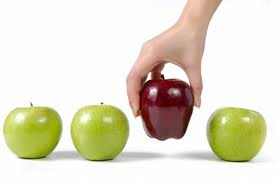
\includegraphics[width=0.25\linewidth]{../Common/images/qa.jpg} 
\end{center}
\end{frame}

\begin{frame}{Examples}
\resizebox{0.9\linewidth}{!}{
\begin{tabular}[t]{@{} p{0.08\linewidth}  
p{0.02\linewidth}  p{0.02\linewidth}  p{0.02\linewidth}   p{0.02\linewidth}  p{0.02\linewidth}  p{0.02\linewidth}     p{0.02\linewidth}  p{0.02\linewidth}  p{0.02\linewidth} p{0.02\linewidth}  p{0.02\linewidth}  p{0.02\linewidth}  p{0.02\linewidth}   p{0.02\linewidth} @{}} \toprule
{\bf mSurf} & 
{\bf $f$}  		& {\bf $l_p$ } 	& {\bf $e_s$ }  	& {\bf $e_{sr}$} & {\bf $e_r$}  & 
{\bf $e_{rr}$} 	& {\bf $e_i$ } 	& {\bf $v_s$ } 	& {\bf $v_r$}  	&  {\bf $v_i$}  & 
{\bf $f_{m}$} 	& {\bf $e_m$ } 	& {\bf $v_m$ } 	& {\bf $\chi_{m}$ } \\ \midrule 

\adjustbox{valign=c}{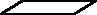
\includegraphics[width=\linewidth]{../Common/images/SimplePlane1.pdf}}  &  
1 & 0 & 4 & 0 & 0 & 0 & 0  & 4 & 0 & 0 & 6 & 12 & 8 & 2 \\ 

\adjustbox{valign=t}{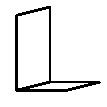
\includegraphics[width=\linewidth]{../Common/images/LPlane1.pdf}}  &  
2 & 2 & 2 & 4 & 1 & 0 & 0  & 4 & 2 & 0 & 8 & 18 & 12 & 2 \\ 


\adjustbox{valign=t}{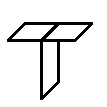
\includegraphics[width=\linewidth]{../Common/images/TPlane1.pdf}}  &  
3 & 2 & 3 & 6 & 1 & 0 & 0  & 6 & 2 & 0 & 11 & 27 & 18 & 2 \\ 

\adjustbox{valign=c}{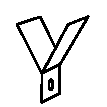
\includegraphics[width=\linewidth]{../Common/images/YwithHolem1.pdf}}  &  
3 & 2 & 3 & 6 & 1 & 0 & 1  & 6 & 2 & 1 & 12  &  30  & 20  & 2 \\ 

\adjustbox{valign=c}{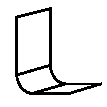
\includegraphics[width=\linewidth]{../Common/images/LwithRoundm1.pdf}}  &  
3 & 2 & 2 & 4 & 2 & 2 & 0  & 4 & 4 & 0 & 10  & 24  & 16  & 2 \\  
\bottomrule
\end{tabular}
}

\vspace{2mm}
As all cases are showing {\bf $\chi_{m}=2$ }  the proposed derivation works !!!


\end{frame}

\begin{frame}{Example of a Practical Shape}
\begin{center}
\resizebox{0.35\linewidth}{!}{
\begin{tabular}[htp]{@{}p{0.48\linewidth} p{0.48\linewidth}@{}} 
{\bf Midsurface} & {\bf Edge Classification} \\
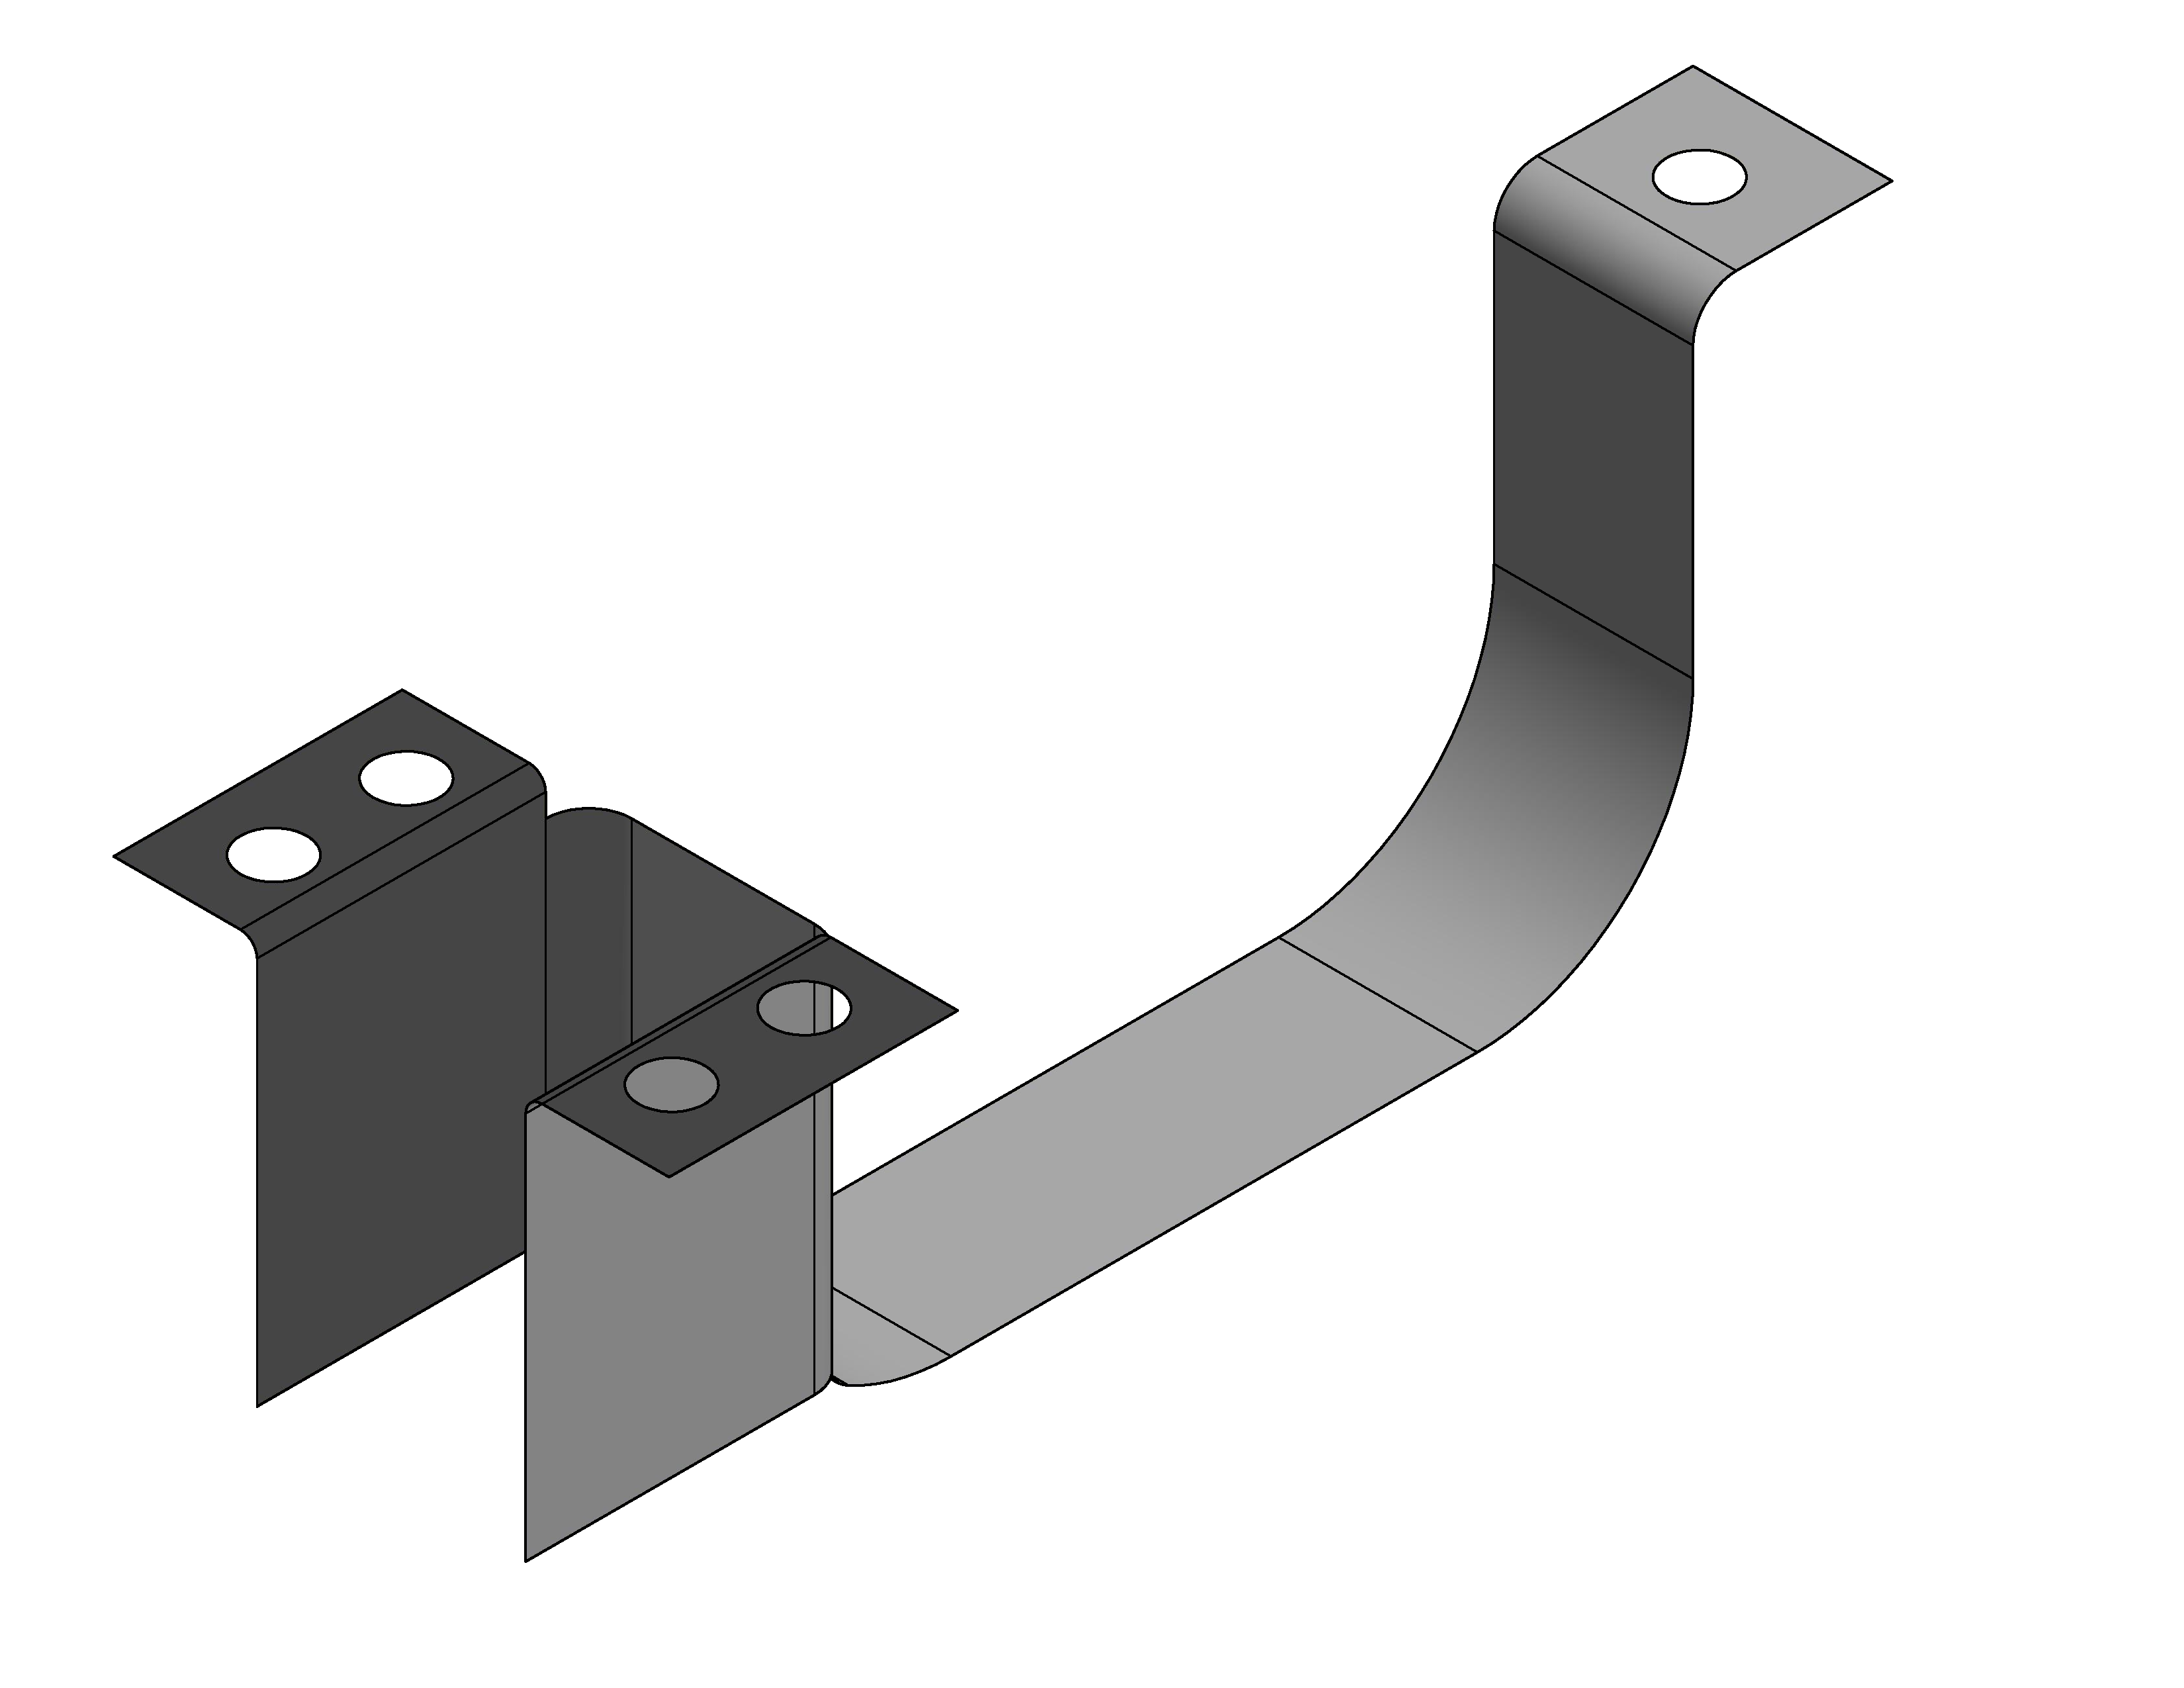
\includegraphics[width=\linewidth]{../Common/images/SimpleBracketMidsurfshaded.pdf} &
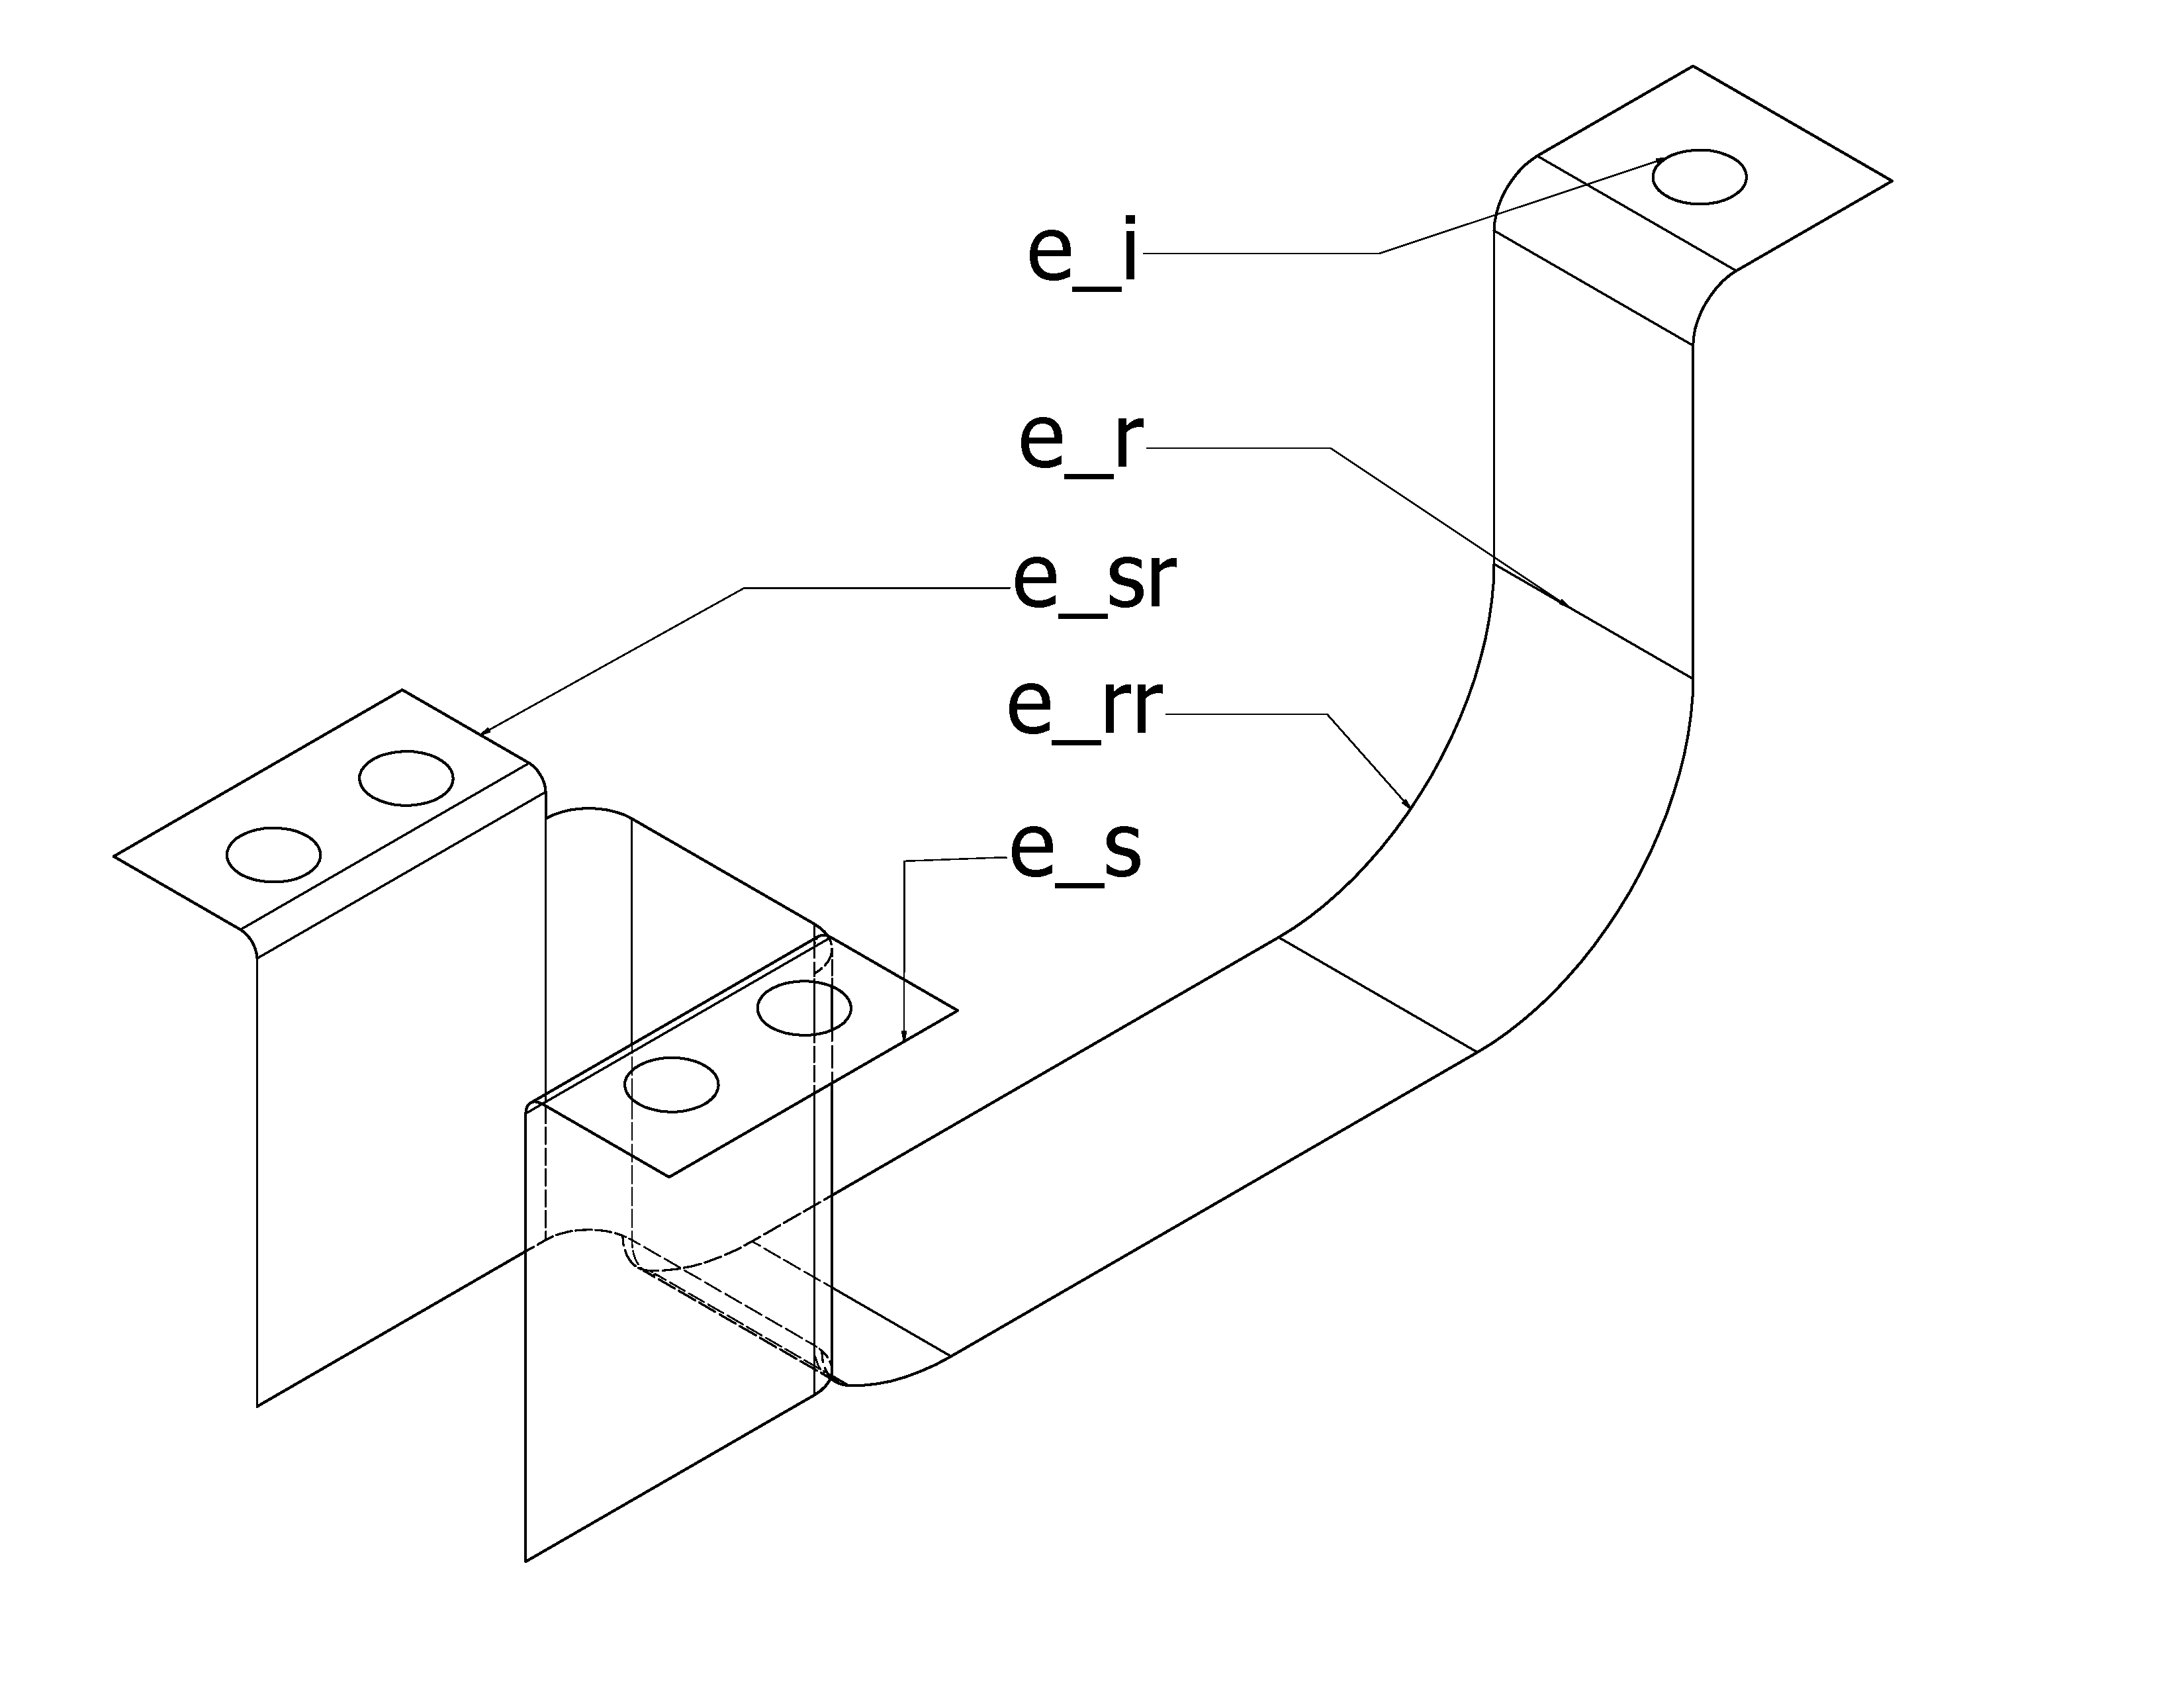
\includegraphics[width=\linewidth]{../Common/images/SimpleBracketMidsurf.pdf}\\
\end{tabular}
}
\end{center}

\begin{itemize}[noitemsep,label=\textbullet,topsep=2pt,parsep=2pt,partopsep=2pt]
%[noitemsep,topsep=2pt,parsep=2pt,partopsep=2pt,label=\textbullet]
\item $f = 15, e_s = 3, e_{sr} = 10, e_r = 14, e_{rr} = 19, l_p = 9 ,e_i=5,v_s = 8,v_r =24, v_i= 5, s=1,h=5,r=5$
\item $f_m = 2f+e_s+ l_p +e_i = 2 \times 15 + 3 + 9 + 5 = 47$
\item $e_m = 2(e_s+e_{sr}+e_{rr}+e_i )+ \sum n_{r} e_{r}+v_s+v_i = 2(3+10+19 + 5)+ (2\times 12 + 4 \times 2)+8+5 = 119$
\item $v_m = 2(v_s+ v_i) + \sum n_{r} v_r=2\times (8 + 5)  + 2 \times 24=74$
\item $s_m =s = 1, h_m = r_i  = 5, r_m = 2r_i = 10$
\item $\chi_{nml} = v-e+f = 32-46+15 = 1$
\item $\chi_{nmr}=s-h+r=1-5+5 = 1$
\item $\chi_{ml} = v_m-e_m+f_m =74-119+47= 2$
\item $\chi_{mr}=2(s_m-h_m )+r_m= 2(1-5)+10 = 2$
%\item Sheet Metal Midsurface Characteristic $\chi_{smm}$\\$=
%e_s+e_i+(2-n_{r} ) e_{r}+e_{sr}/n_{r} $\\$=v_s+(2-n_{r} ) v_{r}+v_i$\\$ 4+0+0+0=4+0+0= 4$
%\item \textbf{Result}: \textcolor{green}{Matches}
\end{itemize}
Predicted solid entities validate the manifold equation ($\chi_{ml} = \chi_{mr} = 2$). 
\end{frame}

\begin{frame}{Limitations}
\begin{itemize}[noitemsep,label=\textbullet,topsep=2pt,parsep=2pt,partopsep=2pt]
\item Topological methods do not capture Geometrical aspects like shape and size.
\item So it is not possible to check whether the midsurface is mimicking the parent shape and is lying midway.
\item Topological entities like faces, edges may get split or merged, without changing the shape. Such operations may give different results for same models, but if we use concept of ``maximal'' entity then this issue gets addressed.
\item Cell decomposition strategies can vary. Say, in case of ``K'', the middle connection point can be represented by one or two interface cells depending on the  definition of a cell. 
\item Splitting done during decomposition may not result in parallelepiped cells. IN case other shapes emerge, special treatment needs to be evolved.
\end{itemize}
\end{frame}